\thispagestyle{endchapter}

\begin{tcolorbox}
\vspace{80pt}

\lettrine{T}{he} pitches in the entrance series to -550 m were derigged with the
ropes left coiled in situ and the metal removed to the Bivouac on top of
the mountain for cleaning and upkeep. The underground campsite was
readied for winter with small reserves of food and fuel being left in
Daren drums, the tent being flipped upside down and the roll mats stood
up to dry. Rope derigged from the \passage{Serpentine} and other pieces
used temporarily for exploration have been left at underground camp for
use in future years, along with a dynamic rope for climbing purposes.

With sufficient caver manpower, we intend to establish a similar deep
camp in 2012 and continue the deep exploration. Though we have
considerable transit times to reach our current pushing targets, the
diverse direction in which they are going suggests that at this point
Camp \passage{X-Ray} is a good a campsite as any other.

We are keen to extend our knowledge of the hydrology of the plateau, and
feel that more extensive dye tracing with a visible agent will be the
best route to understanding both the passage of streams within the cave,
and (with larger quantities of dye) identify the resurgence. Due to the
sensitive location of \passage{Migovec} in the \passage{Triglav national park} and as the
potential drinking water source for a considerable number of local
settlements, this has to be carried out with full support and agreement
of local government agencies \& population. As such, putting together a
scheme of work \& organising permission may require a considerable
amount of time.


\end{tcolorbox}
	\backgroundsetup{	scale=1.1,
        color=black,
        opacity=1,
        angle=0,
        contents={%
                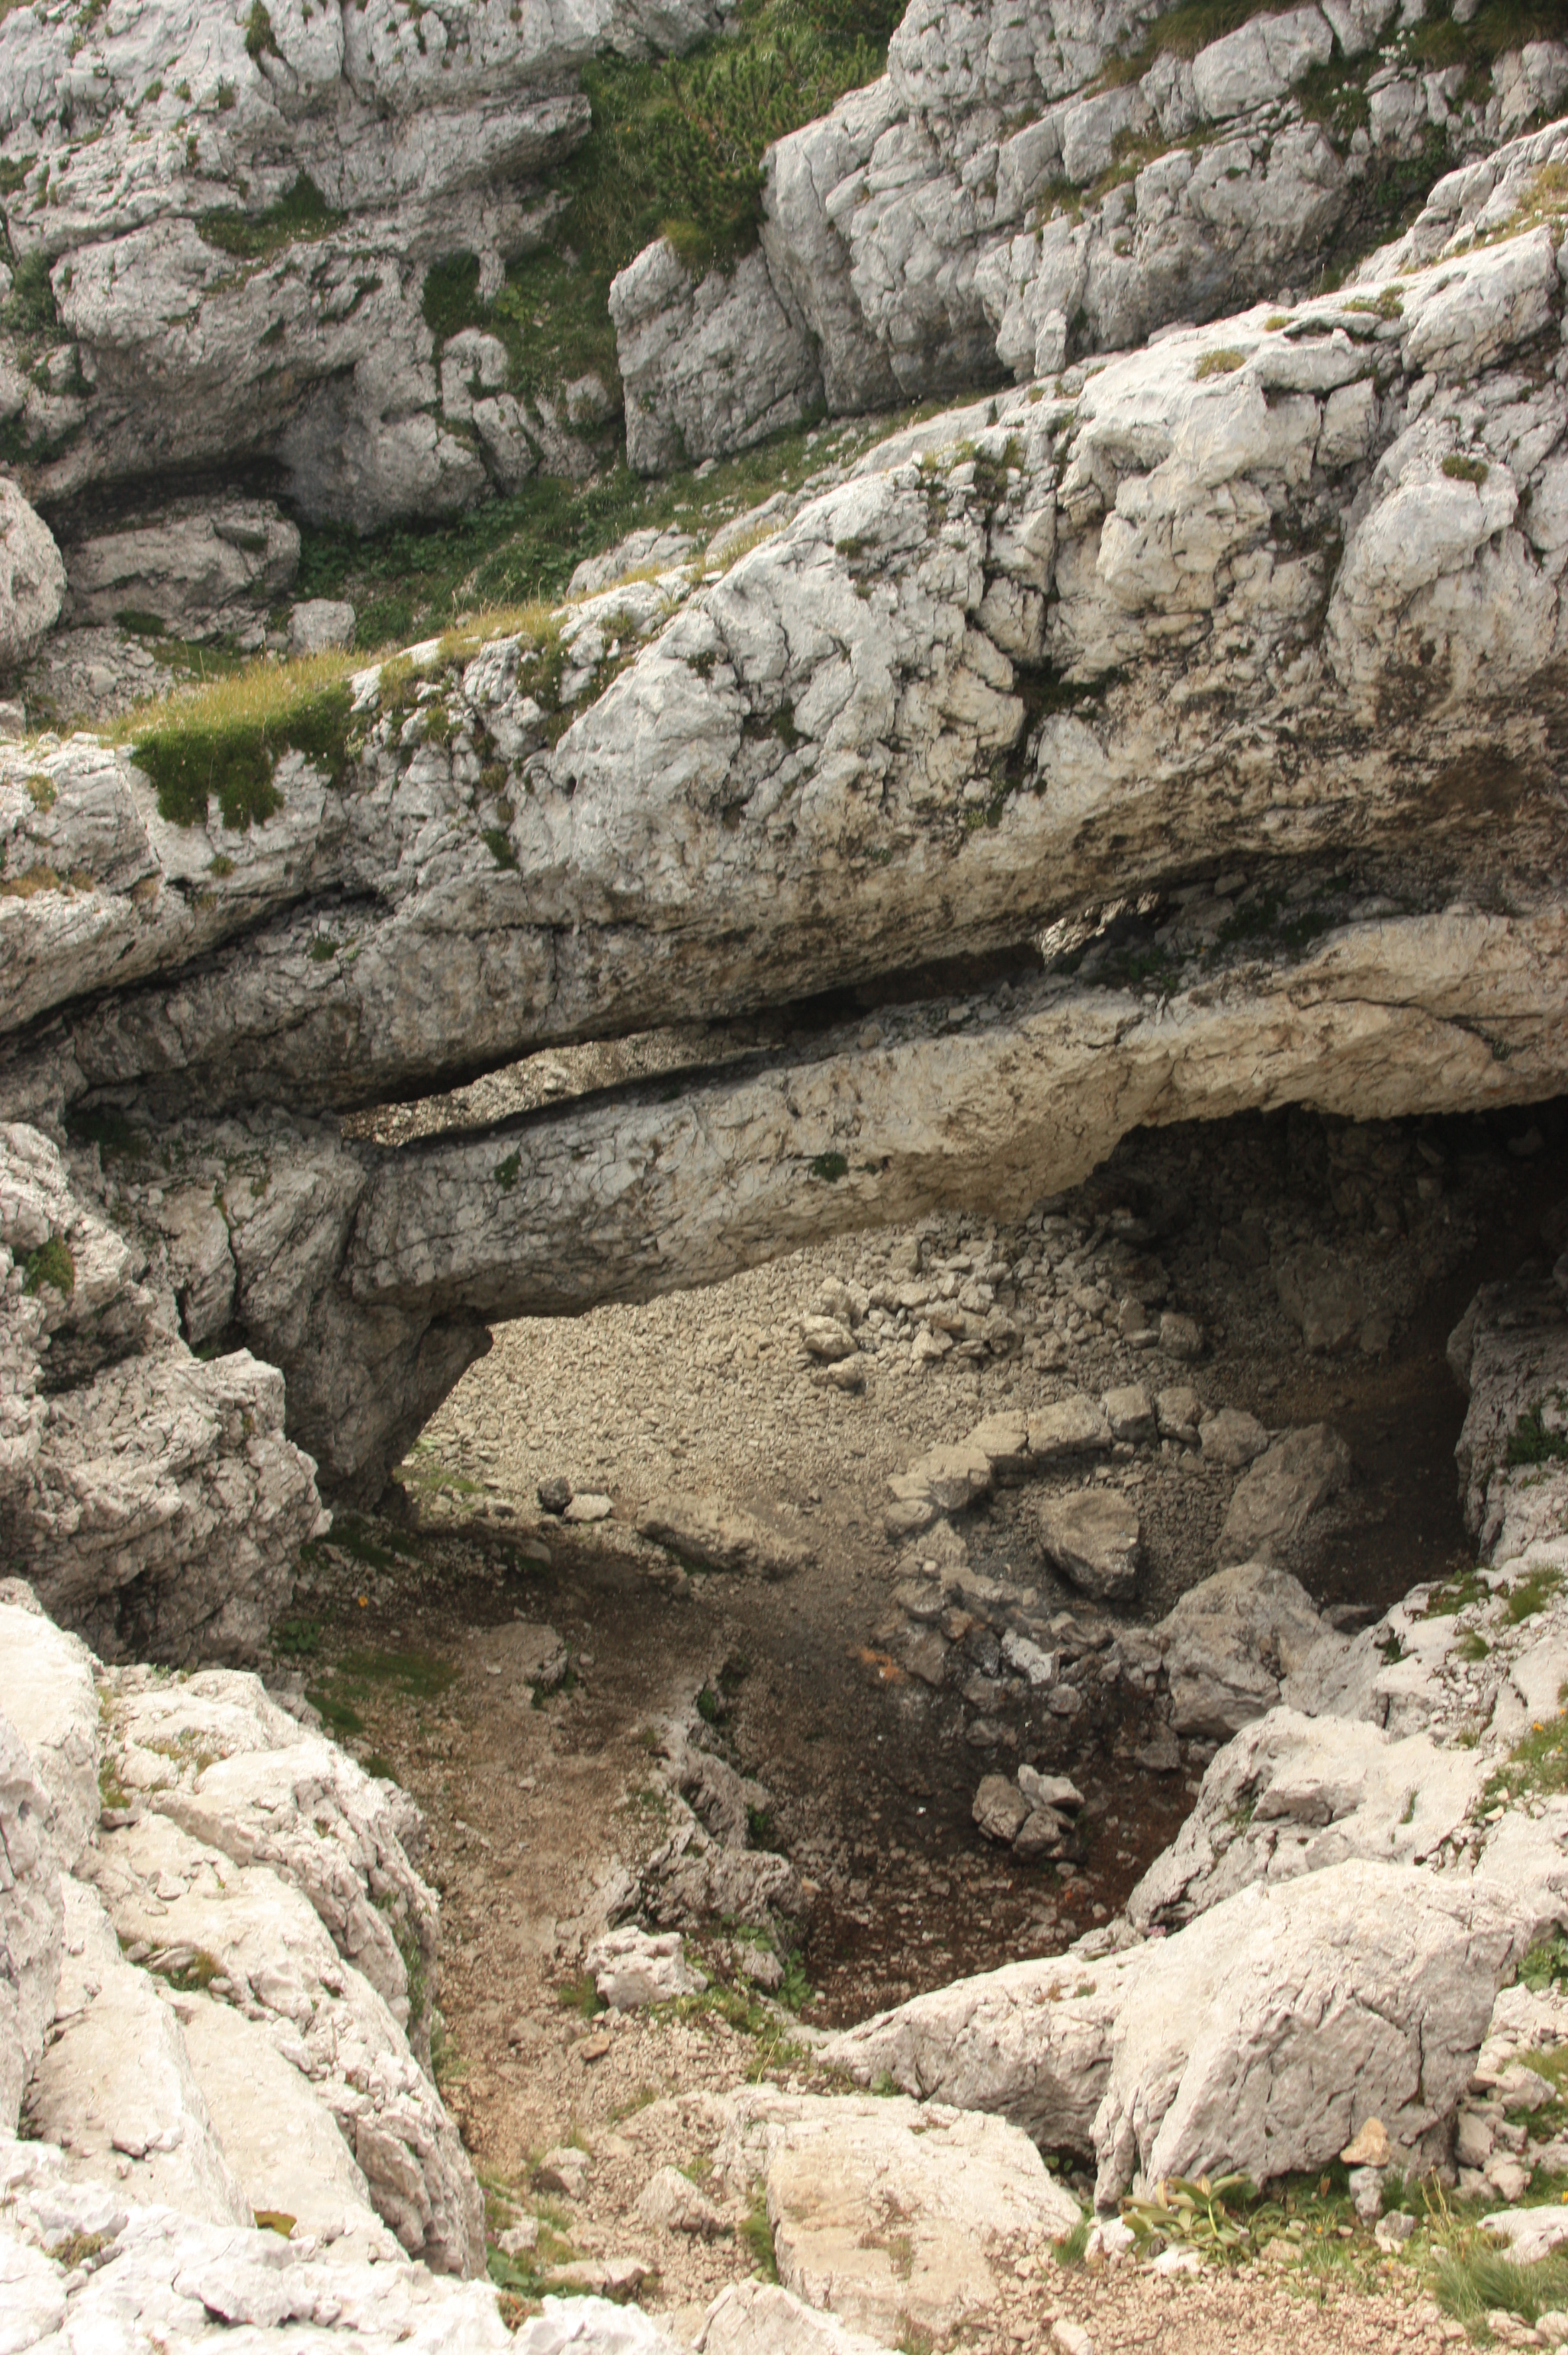
\includegraphics[height=\paperheight]{2011/outro/2011-08-11-15.00.33-Gergely Ambrus-Canon450D-IMG_1384-Mountain Derig--orig.jpg}
        }
	}
\BgThispage
